\section{Stabilität}
    \subsection{Stabilitätsprobleme}
        Stetiger oder plötzlicher Übergang zu stabilen aber meistens unerwünschten deformierten Zuständen.\vspace{-1mm}
        \begin{itemize}
            \item Bei welcher Last findet der Übergang statt?
            \item Wie sieht das Deformationsbild aus?
        \end{itemize}
        \begin{center}
            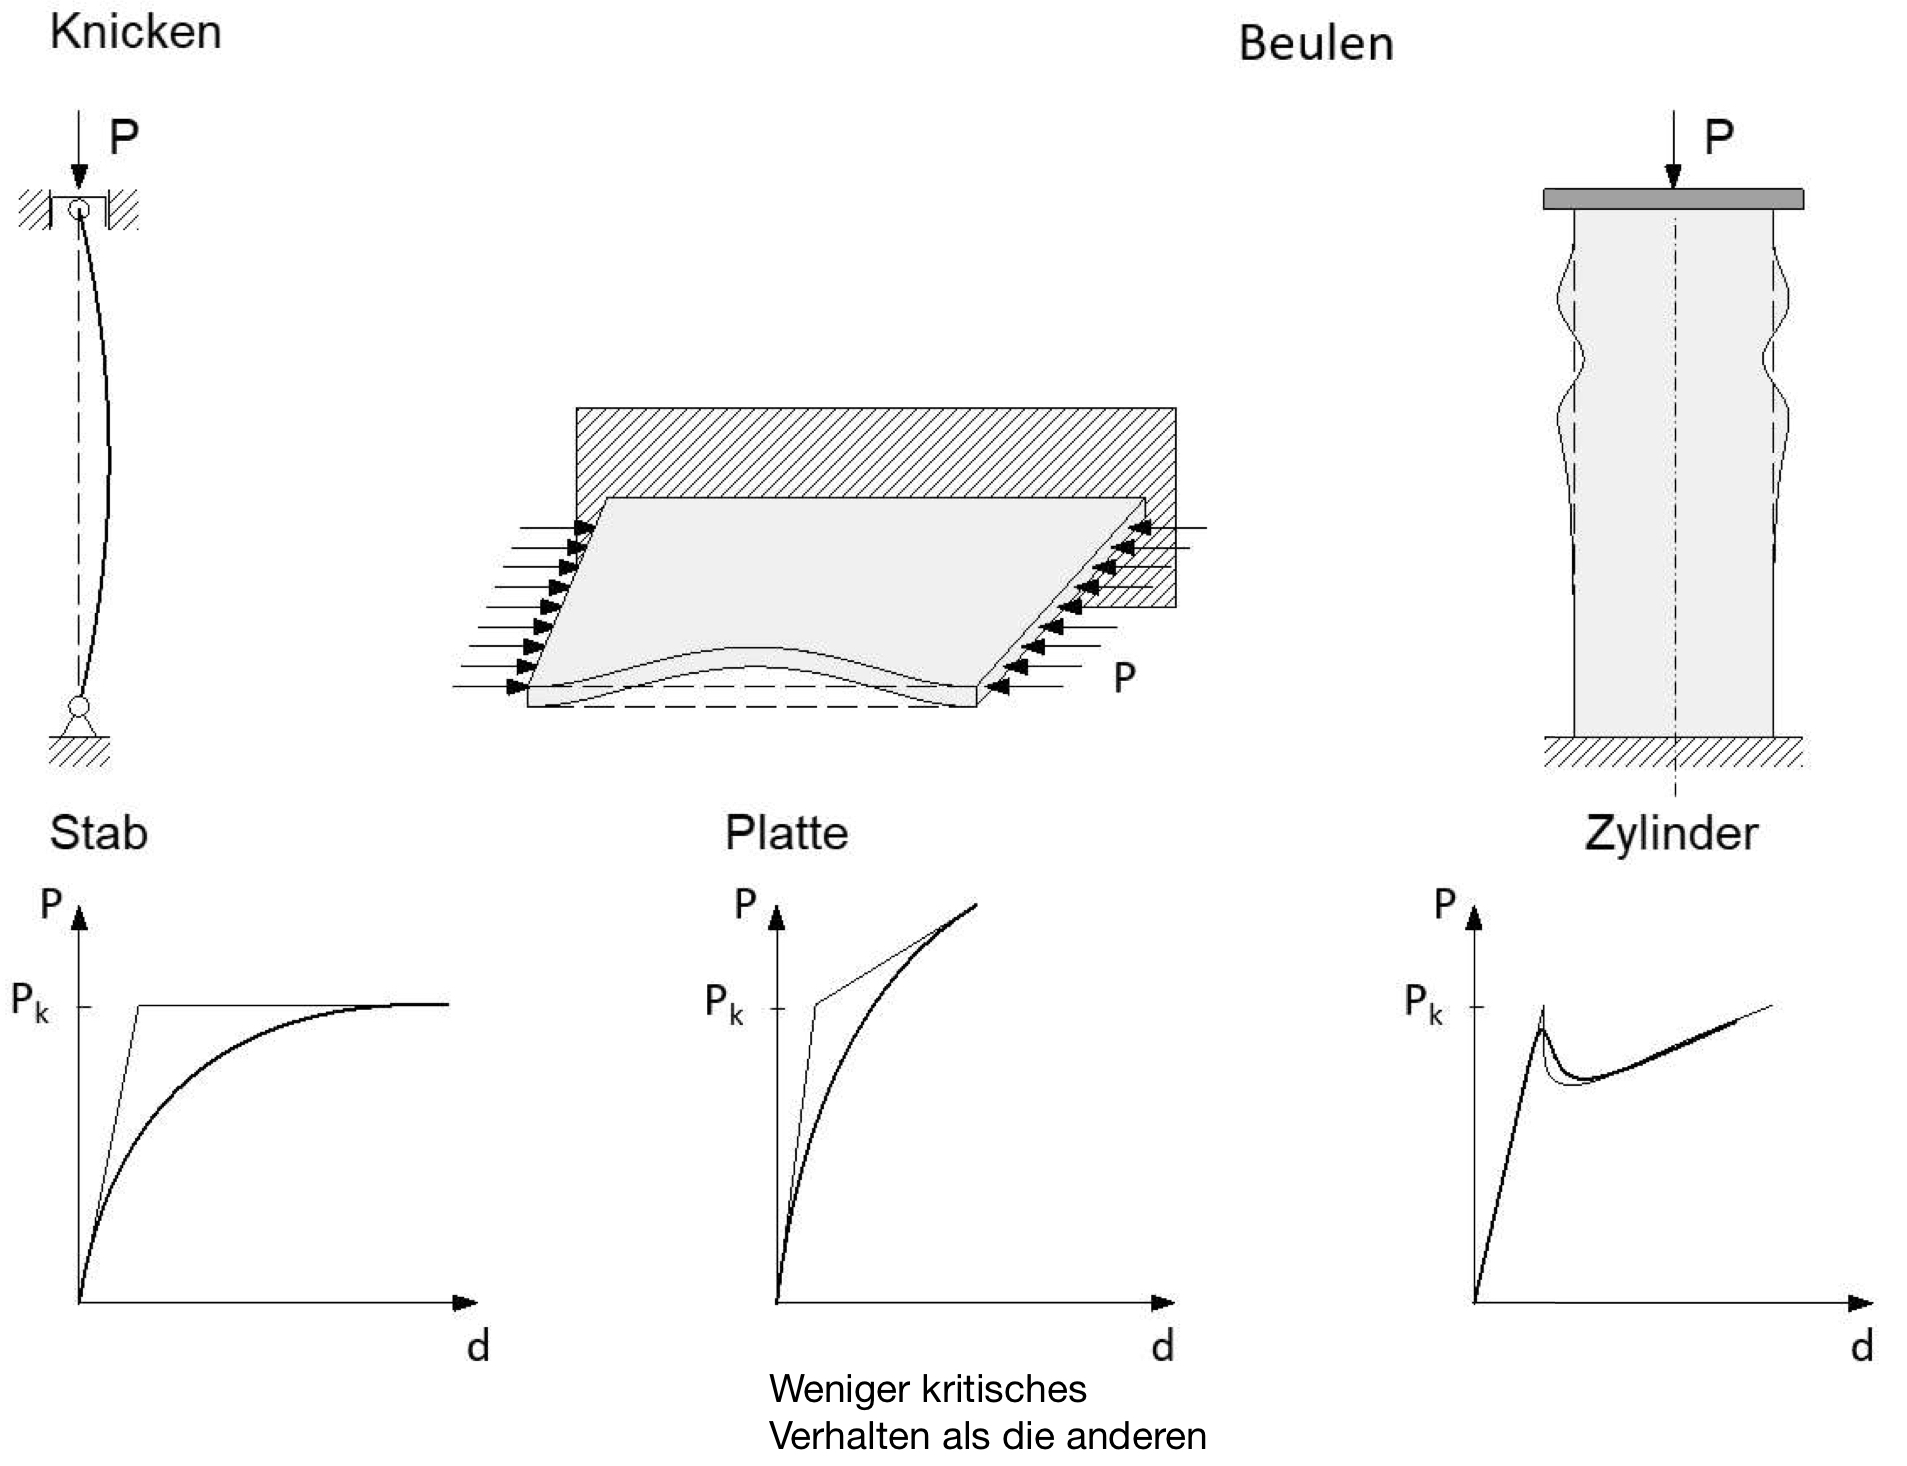
\includegraphics[width=0.7\linewidth , height= 30mm]{09/stability.jpeg}
        \end{center}
    \subsection{1D-Stabilitätsproblem}
        Balken axial belastet, an den Enden axial geführt (oben) und gelenkig gelagert (unten).
        \begin{center}
            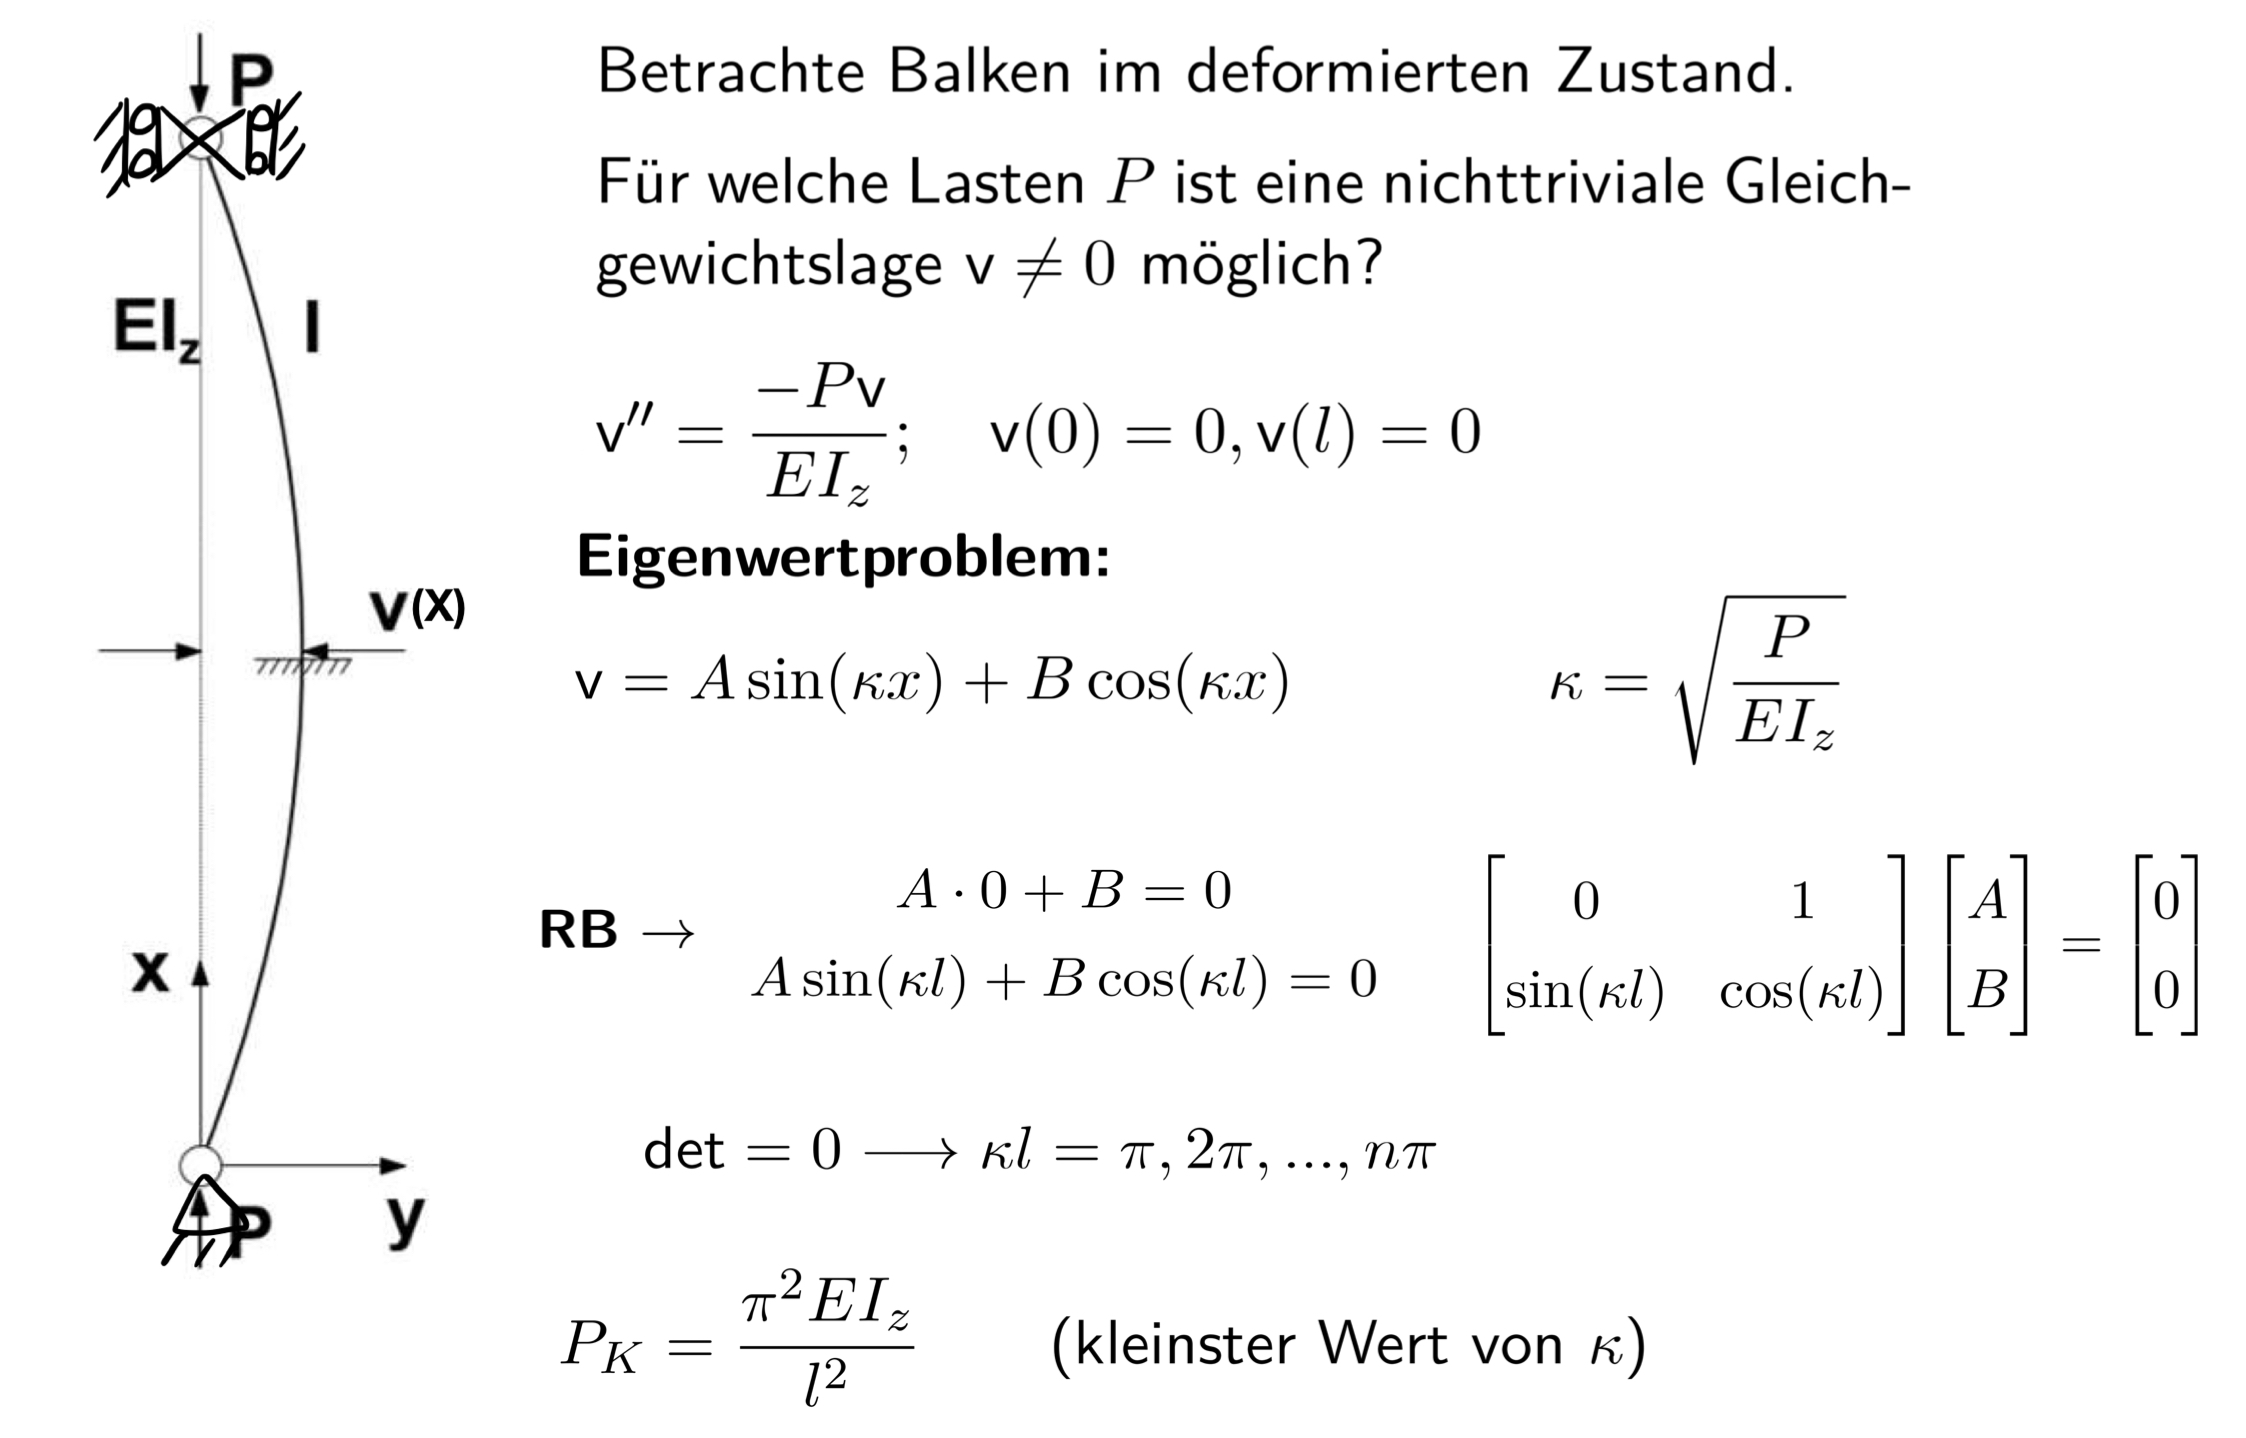
\includegraphics[width=0.9\linewidth,height=45mm]{09/1d.jpeg}
            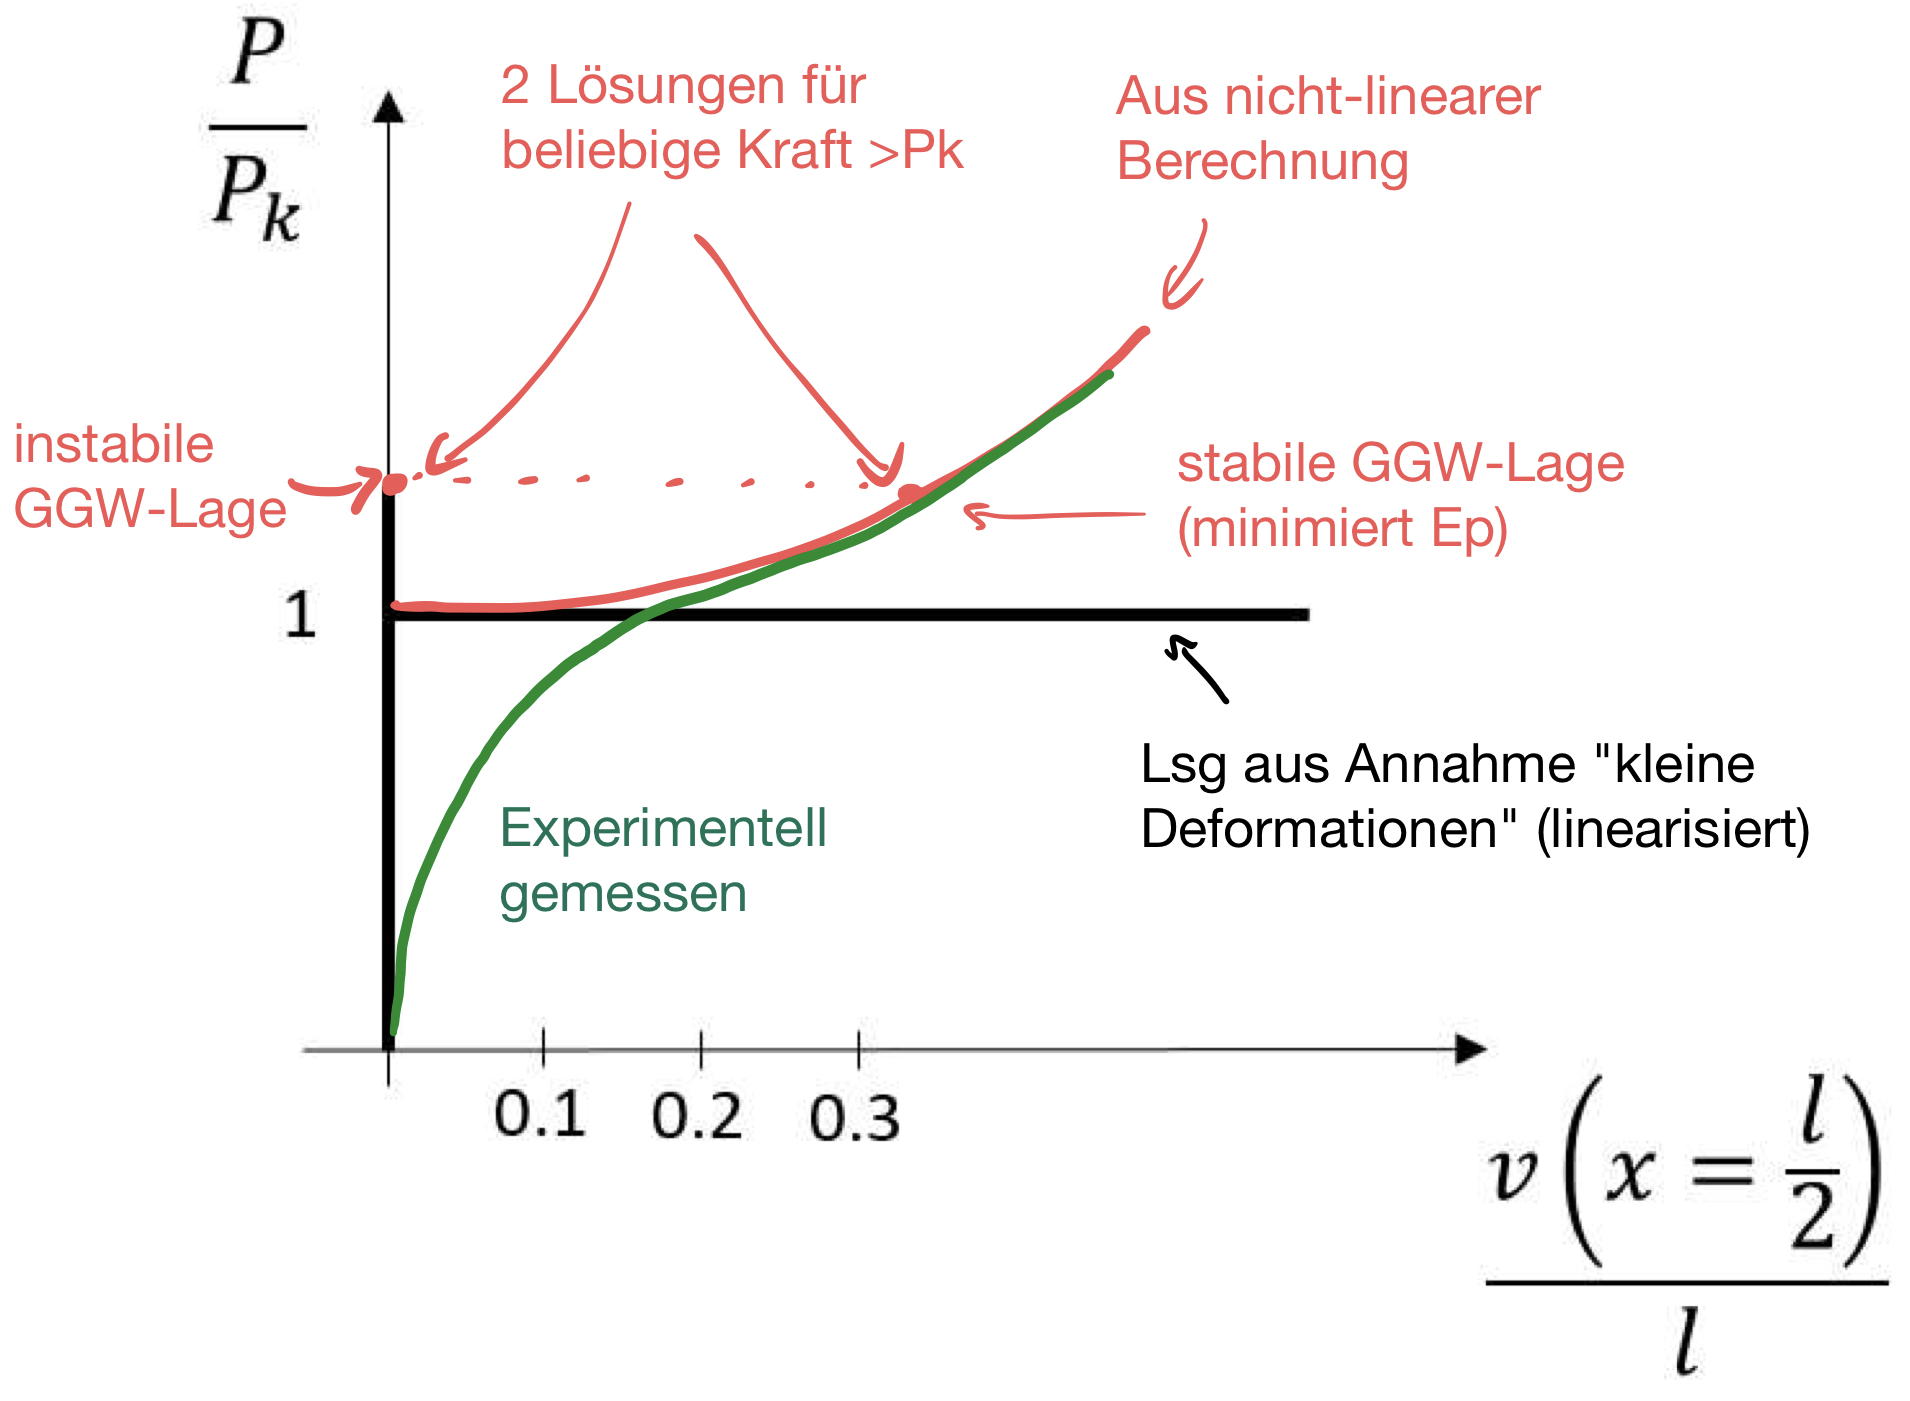
\includegraphics[width=0.85\linewidth, height=45mm]{09/1d-graph.jpeg}
        \end{center}
        Balken einer Seite eingespannt \& andere Seite los.
        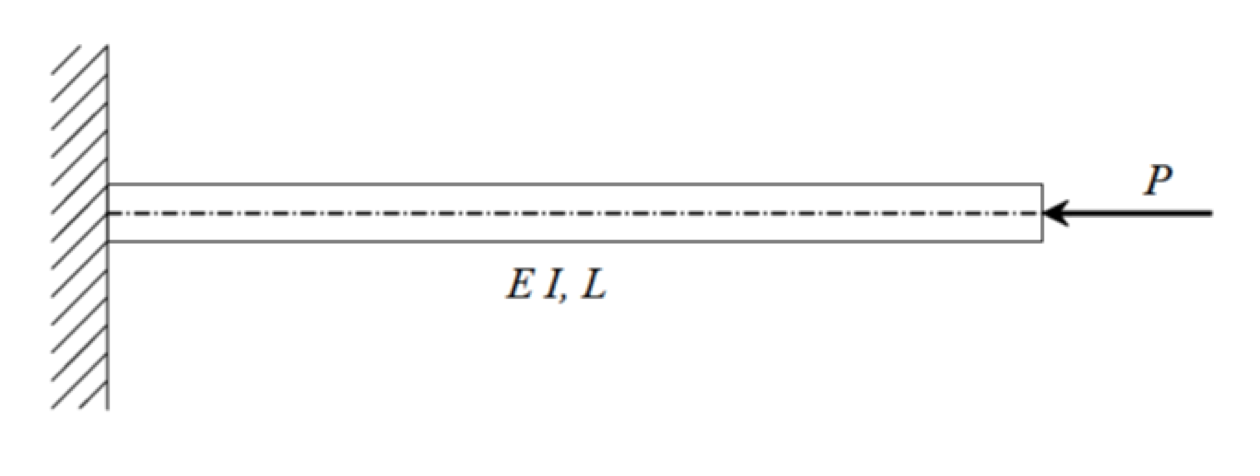
\includegraphics[width=0.6\linewidth]{09/uebung.png}
        \vspace{-17mm}
        \begin{flushright}
        $\displaystyle P_k=\frac{\pi^2EI_z}{4L^2}\qquad\qquad$
        \end{flushright}
        \vspace{7mm}
        
        \begin{comment}
        \subsubsection{Plastifizieren vor Knicken}
            $P_{plast} \leqslant P_k $
        \end{comment}
    \subsection{System mit 1-Freiheitsgrad}
        \TODO{}